\cleardoublepage
\chapter{Produksjon av CMS og nettsted}
\label{chap:implementation} 

% \meta{
% Her skal det beskrives hvordan man faktisk produserte resultatene i prosjektet, og viktigst, beskrive selve produktet. Hvilke verktøy brukte man, hvordan foregikk produksjonen, etc. Utformingen av dette kapittelet avhenger helt klart av type prosjekt.
% }

I dette kapittelet skal vi presentere resultatene i prosjektet og beskrive CMS og nettstedet. Her vil vi også presentere hvilke verktøy vi endte opp med å bruke og hvordan selve produksjonen foregikk.

\section{Verktøy}
Vi endte opp med å bruke flere verktøy enn beskrevet i  \ref{sec:technologies}. 
I tillegg til hovedverktøyene ble følgende verktøy og teknologier benyttet:

\subsection{GNU/Linux}
GNU/Linux er en familie med Unix-lignende operativsystemer som baserer seg på Linux-kjernen \cite{kernel_org} og en del programvare fra GNU-prosjektet \cite{gnu_org}. I denne familien finner vi blant annet Ubuntu, Debian, Fedora, Red Hat Linux og Arch Linux.

I dette prosjektet blir GNU/Linux benyttet som operativsystem på serveren som \q{hoster} back-end.

\subsection{MySQL}
MySQL \cite{oracle2019am} er et databasestyringssystem med åpen kildekode.

Prosjektets database er en MySQL-database.

% \subsection{Let’s Encrypt}
% Let’s Encrypt \cite{le2019ale} er en gratis og åpen sertifikatautoritet som gir ut X.509-sertifikater for kryptering av transportlaget. Tjenesten leveres av ISRG (Internet Security Research Group).

% Studentgruppen har benyttet Let's Encrypt til å lage TLS-sertfikater\footnote{Se avsnitt \ref{sec:analysis-security-tls}}.

\subsection{Node.js}
Node.js er et servermiljø med åpen og gratis kildekode. Node.js kan kjøre på ulike plattformer (Windows, Linux, Unix, Mac OS X) og bruker JavaScript på serveren \cite{w3schools2019win}. I tillegg kan Node.js generere dynamisk sideinnhold og opprette, åpne, lese, skrive, slette og lukke filer på serveren. I tillegg kan Node.js legge til, slette og endre data i databasen.

Vi har brukt Node.js for å kunne kjøre verktøy knyttet til utvikling av front-end.

\section{Tilhørende teknologier og begreper}
Ved å bruke verktøyene som har blitt presentert benyttes også noen tilhørende teknologier. Disse blir presentert videre i dette kapittelet. 

\subsection{Git}
Git \cite{TechTarget} er et system for versjonskontroll. Et versjonskontrollsystem blir hovedsaklig brukt under utvikling av software og nettsteder. Det kan også brukes til andre type prosjekter som grafisk design og skriving av dokumenter.

Ved å bruke Git har vi fått en historikk over alle endringer, samt en sikkerhetskopi av alle versjoner av filene. En annen fordel ved å bruke Git er at det blir enklere å samarbeide med hverandre, uten å måtte tenke på at alle må sitte på nyeste versjon av filene.

% \subsection{Github}
% GitHub.com er et nettsted for å hoste git repositories, og blir mye brukt for \q{Open Source}-prosjekter. 

% Github \cite{TechTarget} er et sentralisert punkt for å samle en brukers repositories. Ved siden av å hoste repositories, lar GitHub brukere dele repositories med hverandre, lage informasjonssider om prosjektet og opprette saker (issues).

% \subsection{HTTP/2}
% HTTP/2 \cite{Belshe2015httpv} er en revisjon av HTTP-nettverksprotokollen. HTTP er et sett med regler for overføring av filer (tekst, grafiske bilder, lyd, video og andre mediefiler). Et av de store målene med HTTP/2 var å tillate multipleksing.

\subsection{REST-API}
Et API (programmeringsgrensesnitt) er et sett med funksjoner, prosedyrer, metoder eller klasser som brukes av dataprogrammer for å be om tjenester fra operativsystemet eller programvare som er på datamaskinen. En programmerer kan bruke API-er til å lage applikasjoner.

REST (Representational State Transfer) er en arkitektonisk stil for programvare. Et REST-API \cite{Masse2011radr} er et API som følger REST-stilen og de begrensninger som REST definerer.

\subsection{Google Analytics}
\label{sec:google-analytics}
Google Analytics \cite{google2019gtk} er en gratis, webbasert tjeneste som gir statistikk og grunnleggende verktøy for analyse av bruksdata, søkemotoroptimalisering og markedsføring.

Dette verktøyet blir av oss brukt til å overvåke hvordan brukerne på nettsiden oppfører seg.

\section{Utviklingen}

Det ble opprettet en \q{Branch protection rule} på back-end repository i Github. Dette gjør at det må kjøres en \q{Code review} før kode kan sendes inn til \q{Master branch}-en. Alle medlemmene på studentgruppen har en egen branch.
Når koden skal commites må det opprettes en pull request, som må godkjennes. Da blir det mulig å luke ut kode som inneholder feil som potensielt kan ødelegge for eksisterende kode.

\section{Back-end}
\subsection{Installasjon og oppsett av Laravel og tilhørende verktøy}
Første steg var å installere package manageren Composer. Deretter kunne siste versjon av Laravel (5.7) settes opp og installeres. Da vi benyttet oss av Composer ble det mulig å installere Laravel med et par kommandoer i terminalen:
\begin{lstlisting}[caption={Installasjon av Laravel med Composer},language=bash]
    composer global require laravel/installer
    laravel new sirkus-media-back-end
\end{lstlisting}

Til slutt måtte vi konfigurere rammeverket slik at det kunne håndtere databasetilkobling, sending av e-post og lagring av opplastede og genererte filer. Laravel samler sine innstillinger i PHP-filer i \q{config} mappen, samt en .env fil som holder på passord og annen sensitiv informasjon vi ikke vil ha i git.

\subsubsection{Database}
Vi begynte med å sette opp tilkobling til databasen. Dette ble gjort ved å først logge inn i MySQL og opprette en bruker og en database. Informasjon for dette ble skrevet inn i .env filen. Se figur under for eksempel:
\begin{lstlisting}[caption={Laravel .env database secrets},language=bash]
    DB_CONNECTION=mysql
    DB_HOST=127.0.0.1
    DB_PORT=3306
    DB_DATABASE=sirkusmedia
    DB_USERNAME=bruker
    DB_PASSWORD=passord
\end{lstlisting}

\subsubsection{Mail}
Etter at databasen var klar for bruk begynte vi å sette innstillingene for e-post. Vi bestemte oss for å bruke Mailtrap\footnote{\url{https://mailtrap.io/}} under utvikling av løsningen. Mailtrap\cite{mailtrap2019setfsad} er en uekte SMTP-server som kan brukes for testing av e-post. Etter å ha registrert bruker hos Mailtrap fylte vi ut følgende informasjon i .env filen:
\begin{lstlisting}[caption={Laravel .env mail secrets}, language=bash]
    MAIL_DRIVER=smtp
    MAIL_HOST=smtp.mailtrap.io
    MAIL_PORT=2525
    MAIL_USERNAME=bruker
    MAIL_PASSWORD=passord
    MAIL_ENCRYPTION=tls
\end{lstlisting}

Når løsningen skal ut i produksjon må det brukes noe annet enn Mailtrap. Sirkus Media kan selv bestemme hva de ønsker å bruke, men systemet er satt opp til bruk av Mailgun\footnote{\url{https://www.mailgun.com/}}.

\subsubsection{Lagring}
Lagring av opplastede og genererte filer foregår på samme server som back-end kjører på. For å sette opp dette kjørte vi en Larvel Artisan kommando:
\begin{lstlisting}[caption={Laravel Artisan kommando for å sette opp lagring av filer}, language=bash]
    php artisan storage:link
\end{lstlisting}
Storage klassen til Larvel gjør at Sirkus Media enkelt kan benytte seg av andre løsninger, som for eksempel Amazon Web Servies S3.

\subsubsection{Laravel Mix}
Laravel Mix\footnote{\url{https://laravel-mix.com/}} var det siste som måtte settes opp før utviklingen kunne starte. Dette er en \textit{wrapper} rundt den populære module bundleren Webpack\footnote{\url{https://webpack.js.org/}}. For å bruke Laravel Mix måtte vi først installere Node.js. Etter Node.js ble installert trengte vi kun å kjøre et par npm-kommandoer:
\begin{lstlisting}[caption={npm-kommando for å sette opp front-end til Laravel}, language=bash]
    npm install
    npm run dev
\end{lstlisting}

For å konfigurere hvilke filer som skal brukes av front-end til Laravel fylte vi ut filen webpack.mix.js:
\begin{lstlisting}[caption={Eksempel på oppsett av webpack.mix.js}]
    const mix = require("laravel-mix");

    mix.sass("resources/sass/app.scss", "public/css").version();
    mix.js("resources/js/app.js", "public/js").version();
    mix.copy("resources/images", "public/images").version();

    mix.browserSync({ proxy: "localhost:8000", notify: false });
\end{lstlisting}

Når vi snakker om \q{front-end til Laravel}, er det ikke snakk om front-end til nettsiden som lages for Sirkus Media, men front-end til CMS-et.
Laravel kommer med en del dependencies til front-end som vi ikke trenger. Alle dependencies defineres i package.json. Følgende dependencies ble fjernet: Bootstrap, jQuery, lodash, Popper og Vue. Det ble kun lagt til en dependency; Shopify sin Draggable pakke. BrowserSync ble også lagt til som en devDependency.

\begin{lstlisting}[caption={Orginal package.json}]
    "devDependencies": {
        "axios": "^0.18",
        "bootstrap": "^4.0.0",
        "cross-env": "^5.1",
        "jquery": "^3.2",
        "laravel-mix": "^4.0.7",
        "lodash": "^4.17.5",
        "popper.js": "^1.12",
        "resolve-url-loader": "^2.3.1",
        "sass": "^1.15.2",
        "sass-loader": "^7.1.0",
        "vue": "^2.5.17"
    },
    "dependencies": {}
\end{lstlisting}

\begin{lstlisting}[caption={Siste package.json}]
    "devDependencies": {
        "browser-sync": "^2.26.3",
        "browser-sync-webpack-plugin": "^2.0.1",
        "cross-env": "^5.1",
        "laravel-mix": "^4.0.7",
        "resolve-url-loader": "^2.3.1",
        "sass": "^1.15.2",
        "sass-loader": "^7.1.0",
        "vue-template-compiler": "^2.6.10"
    },
    "dependencies": {
        "@shopify/draggable": "^1.0.0-beta.8",
        "axios": "^0.18.0"
    }
\end{lstlisting}
Den eneste grunnen til at vue-template-compiler ligger som en dependency her, er fordi siste versjon av Laravel Mix ikke kjører uten.

\subsection{Modeller og database migrations}
Definering av modeller og migrasjon filer til databasetabellene var det første som ble gjort etter konfigurering av rammeverket.
Modeller lagde vi ved å skrive følgende Larvel Artisan kommando i terminalen:
\begin{lstlisting}[caption={Laravel Artisan kommando for oppretting av modell og migration},language=php]
    php artisan make:model Modelnavn -m
\end{lstlisting}
Parameteret \q{-m} i kommandoen over brukes for å opprette en migration-fil for modellen. Det er også mulig å opprette migration-fil etter å ha lagd en modell:
\begin{lstlisting}[caption={Laravel Artisan kommando for oppretting av migration fil},language=php]
    php artisan make:migration migration_file_name
\end{lstlisting}
Etter at modellene og migration filene er opprettet kan man definere forhold mellom modellene (gjøres i modell filen), samt databasetabell for hver modell (gjøres i migration filen).
Når migration filene er ferdig definert kan man kjøre migration ved å skrive følgende kommando i terminalen:
\begin{lstlisting}[caption={Laravel Artisan kommando for å kjøre migration},language=php]
    php artisan migrate
\end{lstlisting}
Etter at migration blir kjørt vil alle tabellene og deres kolonner bli opprettet i MySQL.
Under er et eksempel på en migration fil
\lstinputlisting[caption={Laravel migration fil}, language=php]{laravel-code-examples/migration.php}

\subsubsection{Eloquent forhold mellom modellene}
Eloquent\footnote{\url{https://laravel.com/docs/5.8/eloquent}} er Laravel sitt ORM, det lar oss definere forhold mellom de forskjellige modellene. Det er ønskelig å definere forhold som f.eks: en forfatter har mange bøker. Når et slikt forhold er definert i modellene til Larvel, lar Eloquent oss hente alle bøkene til forfatteren med kode som dette: \lstinline[language=PHP]{$author->books}.

For å definere slike forhold brukte vi de innebygd metodene til Laravel som: belongsToMany, hasOne, belongsTo og hasMany. For eksempel av bruk, se følgende kode:
\lstinputlisting[caption={Laravel modell med et forhold}, language=php]{laravel-code-examples/model-relationship.php}

\subsubsection{Test av migration filer}
Første gang vi kjørte migration dukket det opp en feil:
\begin{lstlisting}[caption={Feilmelding i Laravel ved kjøring av migration},language=PHP]
Illuminate\Database\QueryException : SQLSTATE[42000]: Syntax error or access violation: 1071 Specified key was too long; max key length is 767 bytes (SQL: alter table `users` add unique `users_email_unique`(`email`))
\end{lstlisting}
Denne feilen viste seg å være relativt vanlig og kom av at vi kjørte en eldre versjon (5.7) av MySQL som ikke støtter datatypen varchar med lengde på 255, når collation til databasen er satt til UTF8MB4. Løsningen her ble å sette standard varchar lengde til 191.
\begin{lstlisting}[language=PHP, caption={Definering av standard varchar lengde i AppServiceProvider.php}]
    <?php

    class AppServiceProvider extends ServiceProvider
    {
        public function boot()
        {
            Schema::defaultStringLength(191);
        }
    }
\end{lstlisting}

\subsubsection{Test av forhold mellom modellene}
Når alle forhold var ferdig definert og migration-filene kjørte uten feil, fylte vi databasen med data for å teste at alle forhold var riktig satt opp. Da støtte vi på en feil relatert til vår bruk av UUID som primærnøkkel i stedet for en inkrementerende integer i flere av modellene. Når vi forsøkte å lagre en modell til databasen fikk vi denne feilen:
\begin{lstlisting}[language=PHP]
    SQLSTATE[HY000]: General error: 1364 Field 'id' doesn't have a default value ...
\end{lstlisting}

Feilen kom av hvordan Laravel har satt opp standardmodellen alle modeller baserer seg på. Vi måtte derfor finne en måte å si at alle modeller som brukte UUID har primærnøkkel av typen string, ikke skal inkrementeres. Samtidig skal det genereres en UUID automatisk ved lagring. Den beste måten vi fant å gjøre dette på var ved å lage en trait. Følgende fil ble opprettet:
\lstinputlisting[caption={Trait for å håndtere UUID for Larvel-modeller}, language=php]{laravel-code-examples/trait-uuid.php}

Nå som trait-en var definert, kunne vi inkludere den i alle modeller som brukte UUID som primærnøkkel. Dette blir vist i koden under. Problemet var dermed løst.
\begin{lstlisting}[caption={Bruk av UUID trait i modell}, language=PHP]
    <?php

    use App\Traits\UsesUuid;

    class User ...
    {
        use UsesUuid;

        ...
    }
\end{lstlisting}

Etter de overnevnte problemene ble løst, støtte vi ikke på noen flere nevneverdige problemer rundt forhold mellom modeller.

\subsection{Oppsett av autentisering}
Med databasen og forhold mellom modeller på plass, var vi klare for å begynne utviklingen av selve CMS-et. Vi bestemte oss for å først sette opp autentisering da dette er enklere å implementere fra starten av, fremfor å gjøre det til slutt.
Laravel gir oss mye hjelp på dette området. Ved å kjøre en kommando settes alt vi trenger opp:
\begin{lstlisting}[language=PHP]
    php artisan make:auth
\end{lstlisting}
Etter å ha kjørt kommandoen over, fikk vi de nødvendige controllere og views for innlogging og registrering av brukere, samt system for tilbakestilling av passord.

\subsubsection{Brukerroller}
Selv om autentiseringen var klar, hadde vi ingen måte å skille rettighetene til de forskjellige brukerene på. Dette er heller ikke funksjonalitet som følger med Laravel. Vi fant derfor en PHP pakke: Laravel-Permission\footnote{\url{https://github.com/spatie/laravel-permission}} fra Spatie. Denne pakken utvider Laravel til å støtte brukerroller og kan installeres med Composer. Laravel-Permission gjør det mulig å opprette roller og knytte rettigheter til hver rolle. Vi definerte kun roller og satte følgende: superadmin, admin, moderator og user.
\begin{itemize}
    \item User endte opp med å ikke bli brukt, ligger forsatt tilgjengelig for å gjøre det enklere å utvide systemet videre.
    \item Moderator har tilgang til å opprette, redigere og slette sider og menyer.
    \item Admin har samme tilgang som moderator og kan i tilleg registrere nye brukere.
    \item Superadmin har tilgang til alt. Det vil si at de i tillegg til å kunne gjøre alt det overnevnte, kan lage komponenter, felter og meny lokasjoner, samt at de kan definere hvilke felter en komponent skal ha.
\end{itemize}


\subsection{API}
Vi definerte et API som lot oss hente data fra CMS-et og bygge front-end. Det ble satt opp en prefix for alle API-forespørsler, slik at systemet kan videreutvikles uten å ødelegge for eksisterende løsninger. Alle forespørsler til API-et må starte med /api/v1.

API-et krever ingen autentisering, men forespørsler tillates kun fra spesifikke \textit{origins}. Når prosjektet settes ut i produksjonsmiljø vil forespørsler kun tillates fra \url{https://sirkusmedia.no} og \url{https://www.sirkusmedia.no}. Dette defineres i .env filen.

Følgende lenker kan hentes ut:
\begin{itemize}
  \item pages - Henter ut en liste med alle sider. Hver side i listen holder følgende: id, slug, link, tittel, bilde, dato den ble opprettet og dato som den sist ble redigert.
  \item pages/\{\{slug\}\} - Henter ut en spesifikk side. Den inneholder data om alle komponentene som er på siden, og verdien til feltene til komponentene.
  \item menus - Henter ut en liste med alle menyer og deres lokasjon.
  \item menus/\{\{ID\}\} - Henter ut en spesifikk meny. Her vil alle linker som menyen har, følge med.
\end{itemize}

\section{Oppsett av chat}
Vi bestemte oss for å sette opp en livechat løsning fra Hubspot\footnote{\url{https://www.hubspot.com/products/crm/live-chat}}. Figur \ref{fig:chat-user} viser hvordan det ser ut for sluttbruker. Figur \ref{fig:chat-admin} viser hvordan det ser ut for administrator.
\begin{figure}[H]
    \begin{center}
        \subfigure[Chat når en bruker kommer inn på nettstedet]{
            \label{fig:chat-init}
            \frame{
\includegraphics[width=0.47\textwidth]{bjornar/chat-init.png}}
        }
        \subfigure[Chat åpnet]{
            \label{fig:chat-open}
            \frame{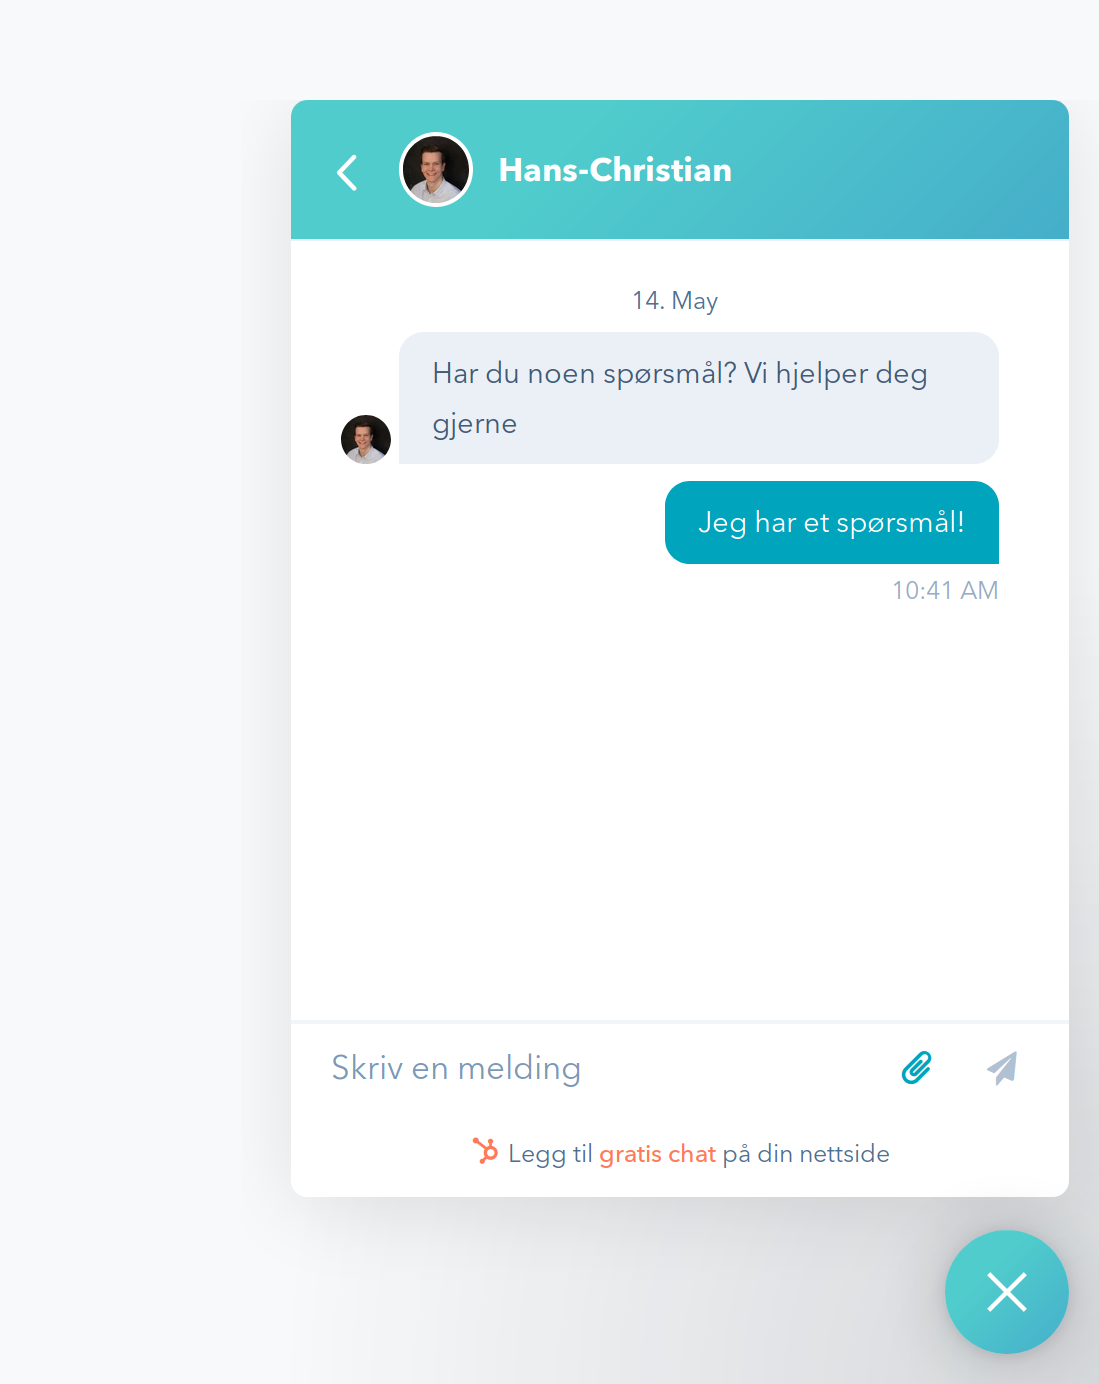
\includegraphics[width=0.3\textwidth]{bjornar/chat-open.png}}
        }
        \label{fig:chat-user}
        \caption{Chat for bruker}
    \end{center}
\end{figure}
\begin{figure}[H]
    \centering
    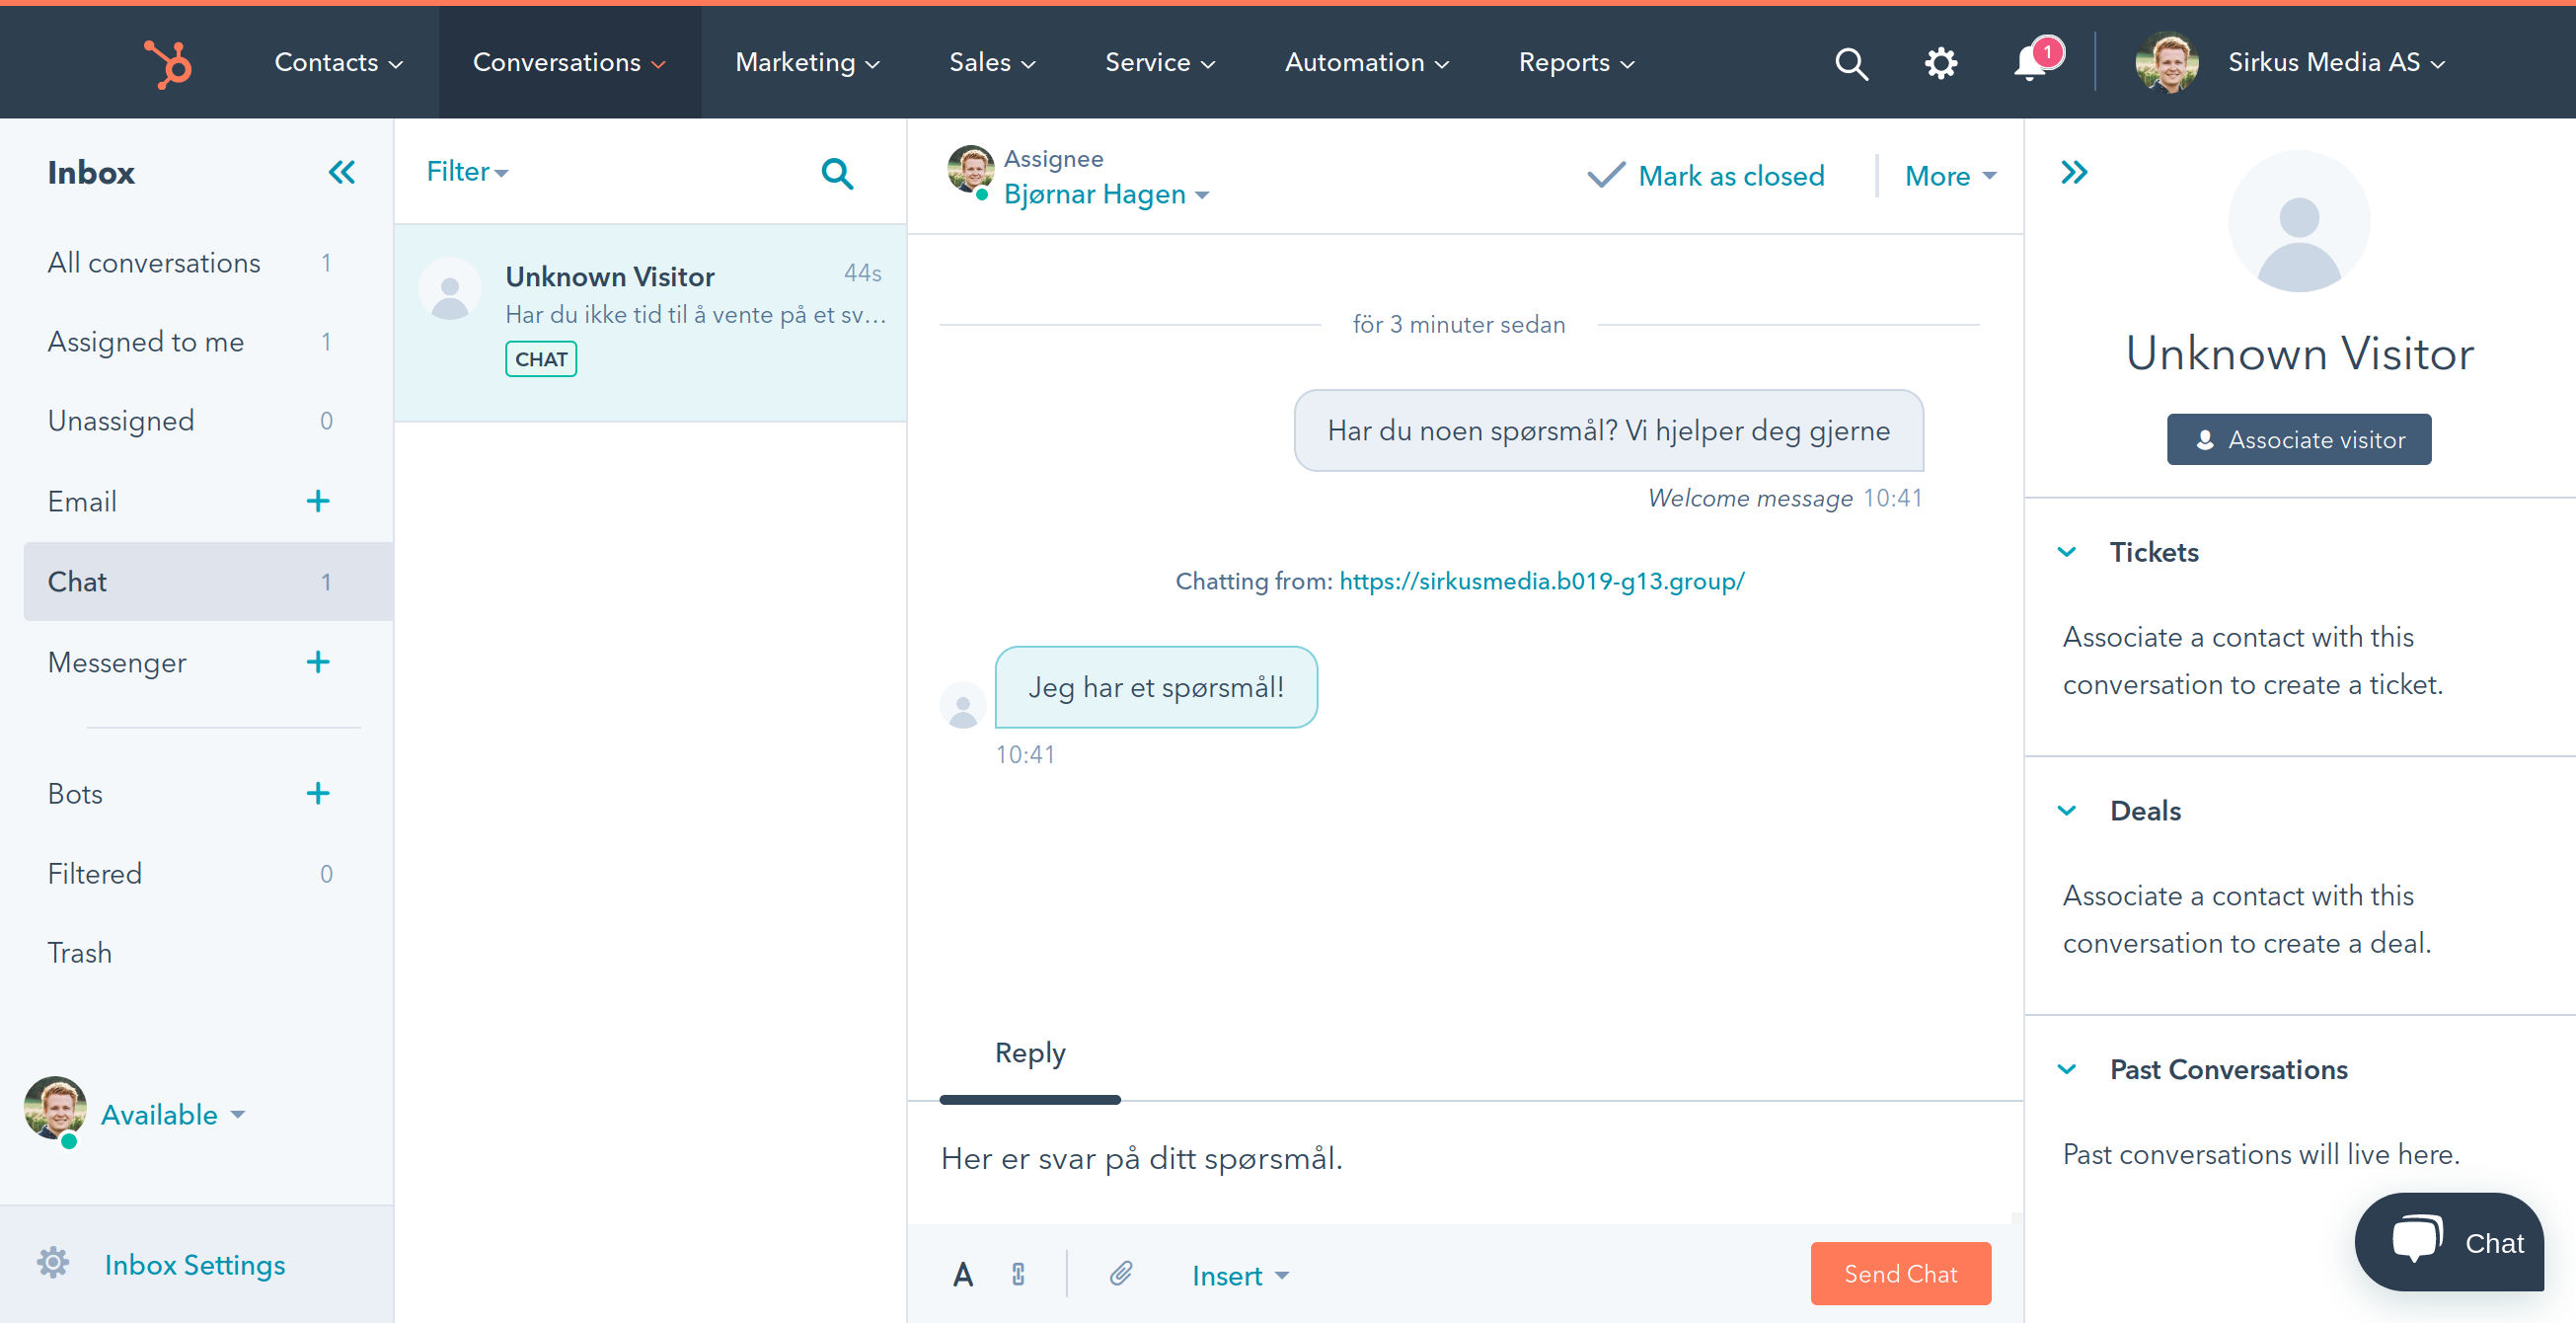
\includegraphics[width=\textwidth]{bjornar/chat-admin.png}
    \caption{Chat for admin}
    \label{fig:chat-admin}
\end{figure}

Vi ønsket at det skulle være lett for Sirkus Media å endre til en annen løsning for chat. Derfor endte vi opp med å legge til ekstra funksjonalitet i CMS'et. Det ble opprettet CRUD for innstillinger (\textit{site\_settings}), som kan hentes ut via API'et på samme måte som \textit{pages}. I innstillingene kan administrator endre hvilket script som blir brukt for chat-løsning, se figur \ref{fig:chat-setting}. Innstillingen for chat hentes ut av front-end, som bruker den til å linke opp til det scriptet som er angitt.
\begin{figure}[H]
    \centering
    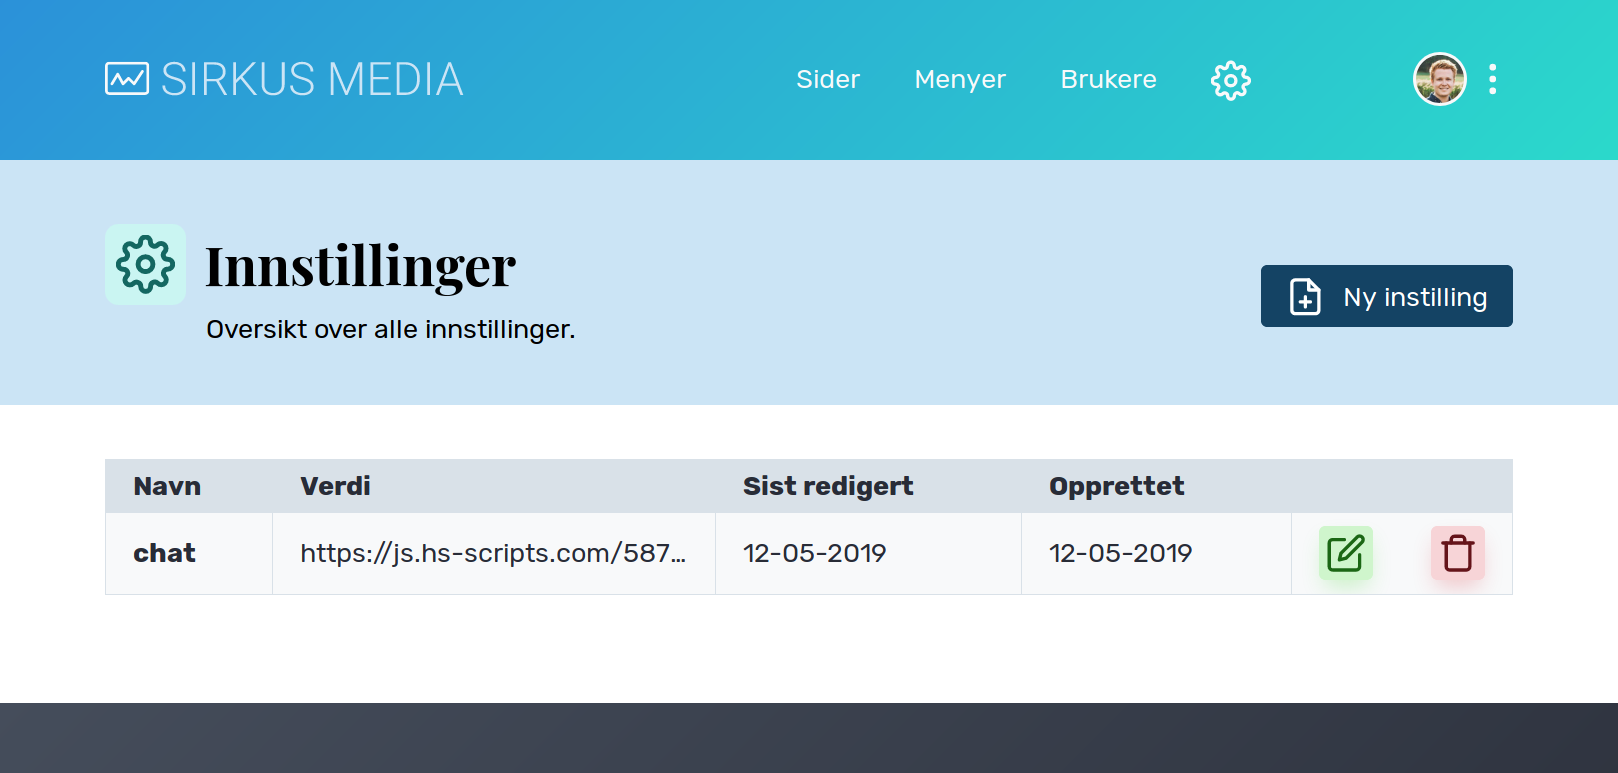
\includegraphics[width=\textwidth]{bjornar/chat-setting.png}
    \caption{Innstilling for chat i CMS}
    \label{fig:chat-setting}
\end{figure}

\section{Oppsett av kontaktskjema}
For kontaktskjema endte vi opp med en løsning fra FormSpree\footnote{\url{https://formspree.io/}}. Det eneste som trengs for å ta i bruk denne, er å sette \textit{action} på kontaktskjema til en URL som dette: \url{https://formspree.io/navn@domene.no}. Hvilken \textit{action} som brukes av kontaktskjema kan styres gjennom CMS'et.

\section{Front-end}
\subsection{Oppsett av React og tilhørende verktøy}

Det første som ble gjort i denne prosessen var å laste ned Node.js\footnote{\url{https://nodejs.org/en/}}. I dette prosjektet blir ikke Node brukt som en back-end tjeneste eller server, men for å kunne kjøre alle verktøy som må til for å kunne utvikle lokalt på datamaskinen. Det var den nyeste versjonen (11.9.0) som ble lastet ned. Deretter ble nettleserutvidelsen React Developer Tools lagt til fra  webstoren til Google Chrome. Det ble også opprettet et repository på Github og lastet ned på maskinen ved hjelp av GitKraken. 
Videre var det nødvendig med et kommandolinjevindu og en teksteditor, valget falt da på kommandolinjevinduet Powershell og teksteditoren Visual Studio Code.

For å sette opp selve React, ble  guiden til react.org for å sette opp en ny React App\footnote{\url{https://reactjs.org/docs/create-a-new-react-app.html\#create-react-app}} fulgt. Her ble det oppgitt at følgende kommandoer må kjøres for å opprette et nytt prosjekt:
\begin{lstlisting}[caption={Oppretting av React App},language=bash]
npx create-react-app my-app
cd my-app
npm start
\end{lstlisting}

Det oppstod problemer når kommandoen \q{npx create-react-app my-app} skulle kjøres, og det kom flere og lange feilmeldinger. Dette måtte undersøkes nærmere, og etter et Google-søk på deler av feilmeldingen ble det oppdaget en sak på Github som omhandlet samme problem\footnote{\url{https://github.com/facebook/react/issues/11933}}.
Løsningen var å installere yarn og create-react-app globalt med yarn. Vi la så til følgende i windows PATH, så kommandoen kunne kjøres:
\begin{lstlisting}
C:\\Users\Line Sharina\AppData\Local\Yarn\bin
\end{lstlisting}
Dette løste problemet og prosessen kunne fortsette. Da ble følgende gjort:

\begin{itemize}
    \item Kjørte \q{npm install} i mappen for prosjektet.
    \item Kjørte \q{npm start} for å starte react serveren.
\end{itemize}

Etter disse stegene begynte planleggingen av de forskjellige komponentene.

\subsection{Planlegging av komponenter}
Komponenter i React kan beskrives som gjenbrukbare biter av kode. En stor fordel med komponenter er at de er mulig å gjenbruke, slik at det ikke lenger er nødvendig å skrive den samme koden flere ganger. 

Ved å se på den godkjente mockupen ble følgende komponenter fastsatt: 
\begin{itemize}
    \item Meny
    \item Header
    \item Resultater
    \item Prosess
    \item Steg i prosess
    \item Kontaktskjema
    \item Footer
    \item Ikon + link
    \item Ikon + tekst
    \item Hvit boks under header. ActionBox
    \item Actions til actionsbox
\end{itemize}

\subsection{Oppretting av components}
Prosessen med oppretting av komponenter startet med å lage en samlemappe som ble kalt \q{components}, som ligger i mappen src. For hver komponent ble det laget en ny undermappe som inneholdt koden til selve komponenten og eventuelt tilhørende stilark.

\subsection{Ruting (Routing)}
Ruting er et mønstergjenkjenningssystem som tar seg av innkommende forespørsler og sender de til spesifikke kontroller-funksjoner. Ruting er ikke innebygd i React. Det ble derfor laget en Router.js-fil i components-mappa. Etter dette ble følgende kommando kjørt:

\begin{lstlisting}[caption={Installering av React ruting},language=bash]
npm install react-router-dom
\end{lstlisting}

Deretter kunne vi importere react-router-dom i filen Router.js:

\begin{lstlisting}[caption={Importering av react-router-dom},language=bash]
import {BrowserRouter, Route, Switch} from "react-router-dom";
\end{lstlisting}

Den foreløpige versjonen av back-end ble lastet ned og lagret lokalt, slik at det ble mulig å teste underveis.

For å kunne snakke og bruke foreløpig backend ble Axios\footnote{Se mer i avsnitt \ref{sec:tool:axios}} benyttet. Hvis etableringen av forbindelsen er vellykket, slik at det har blitt opprettet kontakt med API via Axios, vil alle svar som ble gitt av back-end bli lagret i en array. 

Deretter ble det satt opp en dynamisk ruting, ved hjelp av en løkke som går igjennom alle eksisterende sider og setter opp linker til disse.

\subsection{Installering av Axios}
Axios blir i vårt system brukt til å sende forespørsler til back-end. Dette biblioteket ble installert ved å kjøre kommandoen under.  Kommandolinjevindu må åpnes i filstilen der mappa til prosjektet er plassert.
\begin{lstlisting}[caption={Installering av Axios},language=bash]
npm install axios
\end{lstlisting}

\subsection{Page components}

Det ble opprettet et objekt som inneholder alle komponentene som er definert i databasen. Ved å loope igjennom alle komponentene til en side, ble det da mulig å sjekke om navnene samsvarte. Hvis de gjør dette, vil det kjøres en løkke som går igjennom alle feltene en komponent inneholder. Til slutt blir alle komponentene til en side, med riktige props\footnote{Props i React brukes til å sende med utvalgt data til en komponent} skrevet ut.  

Før det ble opprettet et objekt som inneholdt alle eksisterende components, ble det forsøkt å kun hente ut angitt komponenter til siden i back-end og så opprette components ut av dette. Da fikk vi følgende feil:
\begin{lstlisting}
<HeaderComponent /> is using incorrect casing. Use PascalCase for React components, or lowercase for HTML elements.
\end{lstlisting}

Feilmeldingen var at komponenten brukte feil casing, noe som ikke var riktig da feilmeldingen viste at \q{\textless HeaderComponent /\textgreater} var skrevet på riktig måte. Etter en del feilsøking, fant vi ingen som hadde løst dette problemet tidligere. Vi endte derfor opp med å opprette objektet som inneholder alle komponentene. 

I tillegg til å finne ut av hvilke komponenter som tilhører siden, må man i tillegg finne ut av hvilke felter som tilhører hvilke komponenter. Dette blir satt i back-end. I løkka som går igjennom objektene ble det derfor lagt til en ny løkke, som går igjennom og lagrer alle tilhørende felter til en komponent i en array. Denne arrayen blir så sendt videre som props i de ulike komponentene.

\subsection{Child components}
I systemet vårt kan en komponent ha flere \q{barn}. Det å ha komponenter som er barn av en komponent gjør at disse har et forhold til hverandre. Da blir det mulig å putte forskjellig innhold inn i en felles seksjon.

\subsection{Felter med samme navn}
Underveis i prosessen ble det oppdaget at hvis en komponent hadde den samme felttypen flere ganger, ville bare den siste verdien bli skrevet ut. En komponent vil ofte bestå av for eksempel flere tekstfelt, og derfor måtte vi finne en måte å løse dette på.

Løsningen ble en betingelsetest der det blir sjekket om samme felttype er til stede flere ganger. Hvis denne blir sann, vil feltene med verdier bli lagt til i en array. 

\subsection{Utskrift av tomme felter}
Videre i prosessen ble det oppdaget at hvis en prop ikke innholdt en verdi, ville feltet fortsatt bli skrevet ut. Dette førte til at nettstedet inneholdt mange tomme HTML-tagger. Brukervennligheten på for eksempel skjermlesere hadde blitt betraktelig dårligere, så derfor måtte dette gjøres om. Løsningen ble å gjøre en betingelse-test på hver prop, for å sjekke om den innholdt en verdi. Da ble det mulig å kun skrive ut om dette var oppfylt.

\subsection{Testing}
For å teste systemet, ble header-komponenten laget. Når denne ble opprettet både i objektet og back-end, ble alle props/feltene som blir mottatt fra komponenten skrevet ut. Dette betydde at Header-komponenten fungerte som den skulle, og vi kunne starte med å legge til resten av komponentene på samme måte. 

Da kunne vi også begynne å style komponentene slik at de ligner mockupen som ble laget.

\subsection{Kompilere SCSS til CSS}
Gruppen har tidligere nevnt at det ble besluttet å bruke SASS til styling. Da er det nødvendig å ha noe som kompilerer fra SCSS til CSS. Dette ble oppnådd ved å følge guiden hos TechCookbook\footnote{\url{https://techcookbook.com/react/use-scss-with-create-react-app}}

Installerte først node-sass ved å kjøre :

\begin{lstlisting}[caption={Installering av node-sass},language=bash]
npm install --save node-sass
\end{lstlisting}

Etter at pakken ble installert, måtte det lages et script som kompilerer fra .scss til .css:

\begin{lstlisting}[caption={Kompliering fra .scss til .css}]
 "build-css": "node-sass src/ -o src/"
\end{lstlisting}
\clearpage

\q{Build-css} tar .scss-filene som finnes i source-mappen samt undermapper og kompilerer dem til .css-filer. .css filen vil bli tilgjengelig i den samme lokasjonen som den originale .scss-filen. Deretter ble det laget et script som kjører \q{build-css} og kompilerer alle eksisterende filer til .css, samtidig som den ser etter forandringer i source-mappen. Den vil altså detektere om det blir gjort endringer i eksisterende .scss filer, eller om det blir lagt til nye. 

\begin{lstlisting}[caption={Script som detekterer scss endringer}]
 "watch-css": "npm run build-css && node-sass src/ -o src/ --watch --recursive"
\end{lstlisting}

En test ble gjort ved å lage en fil som het "header.scss" og satte bakgrunnsfargen til rød. Dette fungerte som det skulle.

\begin{lstlisting}
 body {
  background-color: red;
}
\end{lstlisting}

\subsection{Styling}
Designet til nettstedet ble stylet ved hjelp av SCSS, og er så lik den godkjente mockupen som mulig. Designet er også responsivt og fungerer derfor like godt på stor skjerm, laptop, nettbrett og mobil. For stylingen ble prinsippet \q{mobil først} benyttet. Dette prinsippet går ut på at utviklingen først skjer for små skjermer, for deretter å skalere opp og gjøre designendringer når det er nødvendig. 

\subsection{Ikoner og illustrasjoner}
Ikonene er hentet fra Feather\footnote{\url{https://feathericons.com/}}. Feather er en ikonpakke med åpen kildekode. Alle illustrasjonene er hentet fra unDraw\footnote{\url{https://undraw.co/}}. På nettsiden til unDraw oppgir de at både private og kommersielle kan bruke og modifisere illustrasjonene gratis\footnote{\url{https://undraw.co/license}}. Siden disse er av filtypen SVG har vi hatt muligheten til å tilpasse fargene på illustrasjonene til å passe designet til nettstedet.

\section{DevOps}
Vi har ikke fått all informasjon som skal på nettstedet eller tilgang til domenet til Sirkus Media. Nettsted og CMS måtte derfor lastes opp på midlertidig domener.
I forbindelse med prosjektet skulle gruppen ha et eget nettsted der det er informasjon om oppgaven og gruppen, samt oppdatering underveis i prosessen. Det ble derfor kjøpt et eget domenet for dette: \url{b019-g13.group}. Vi bestemte oss for å bruke det samme domenet. Det ble opprettet et subdomene hver for front-end og back-end: \url{sirkusmedia.b019-g13.group} og \url{api.b019-g13.group}.

Front-end ble lastet opp og kan styres via Netlify\footnote{\url{https://www.netlify.com/}}. Back-end skulle i utgangspunktet settes opp på en virtuell server hos DigitalOcean\footnote{\url{https://www.digitalocean.com/}}, som vi selv satt opp med LEMP. Vi endte opp med en litt annen løsning, der alt settes opp og styres gjennom Laravel Forge\footnote{https://forge.laravel.com/} og oppdateres med Envoyer\footnote{\url{https://envoyer.io/}}. Oppsettet kjører forsatt på en VPS hos DigitalOcean, men vi trengte ikke lenger å sette opp LEMP.

\section{Første versjon av database, CMS og nettsted}
Det ble noen avvik fra den planlagte databasen. Databasen ble derfor mer optimalisert og bedre tilpasset det oppsettet vi ønsket, se figur \ref{fig:first-version-db} og \ref{fig:first-version-db-other}.

\begin{figure}[H]
    \centering
    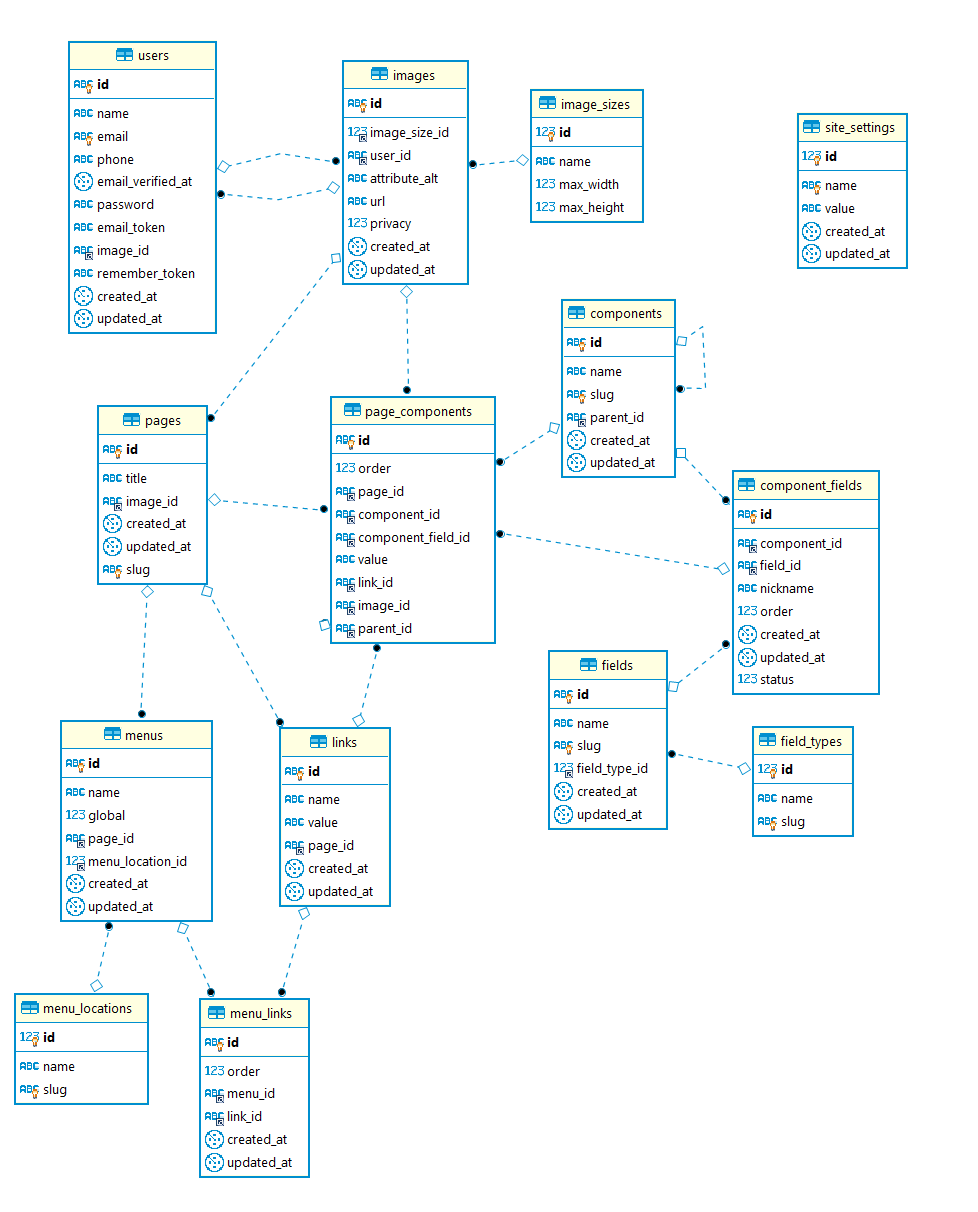
\includegraphics[width=\textwidth]{bjornar/db-endelig.png}
    \caption{Første versjon av databasen - hovedtabeller}
    \label{fig:first-version-db}
\end{figure}

\begin{figure}[H]
    \centering
    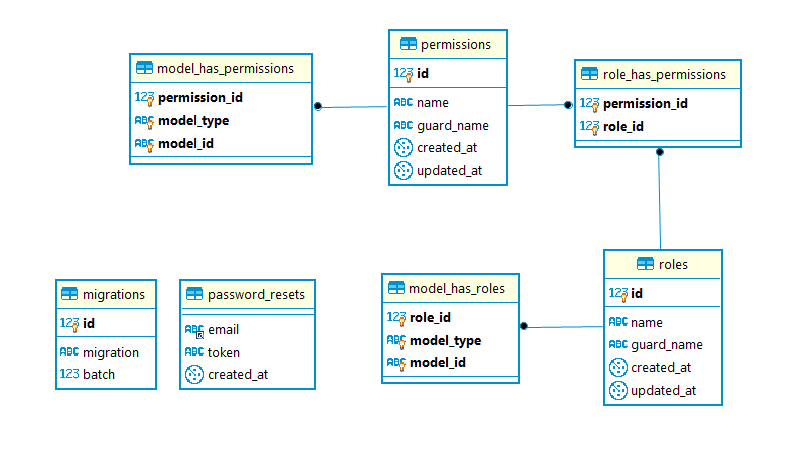
\includegraphics[width=\textwidth]{bjornar/db-endelig-annet.png}
    \caption{Første versjon av databasen - andre tabeller}
    \label{fig:first-version-db-other}
\end{figure}

CMS-et endte opp med å bli som vi planla i avsnitt \ref{sec-planning-cms}. Det var kun en ekstra funksjonalitet som ble lagt til, muligheten til å gi kallenavn til felter som tilhører komponenter. Dette gjør det enklere for sluttbruker å redigere sider. En funksjonalitet som ble diskutert under planlegging, men aldri skrevet ned var en bildevelger. Felter som er av typen bilde, har en referanse til Image-modellen. For å sette verdien til dette feltet på riktig måte, trenger man en ID til et bilde i \q{images}-tabellen. Alt dette tar bildevelgeren seg av, samt at den gjør det enkelt å laste opp nye bilder. Figur \ref{fig:first-version-cms} viser første versjon av CMS-et, og \ref{fig:media-picker-cms} viser bildevelgeren til CMS-et.

\begin{figure}[H]
    \centering
    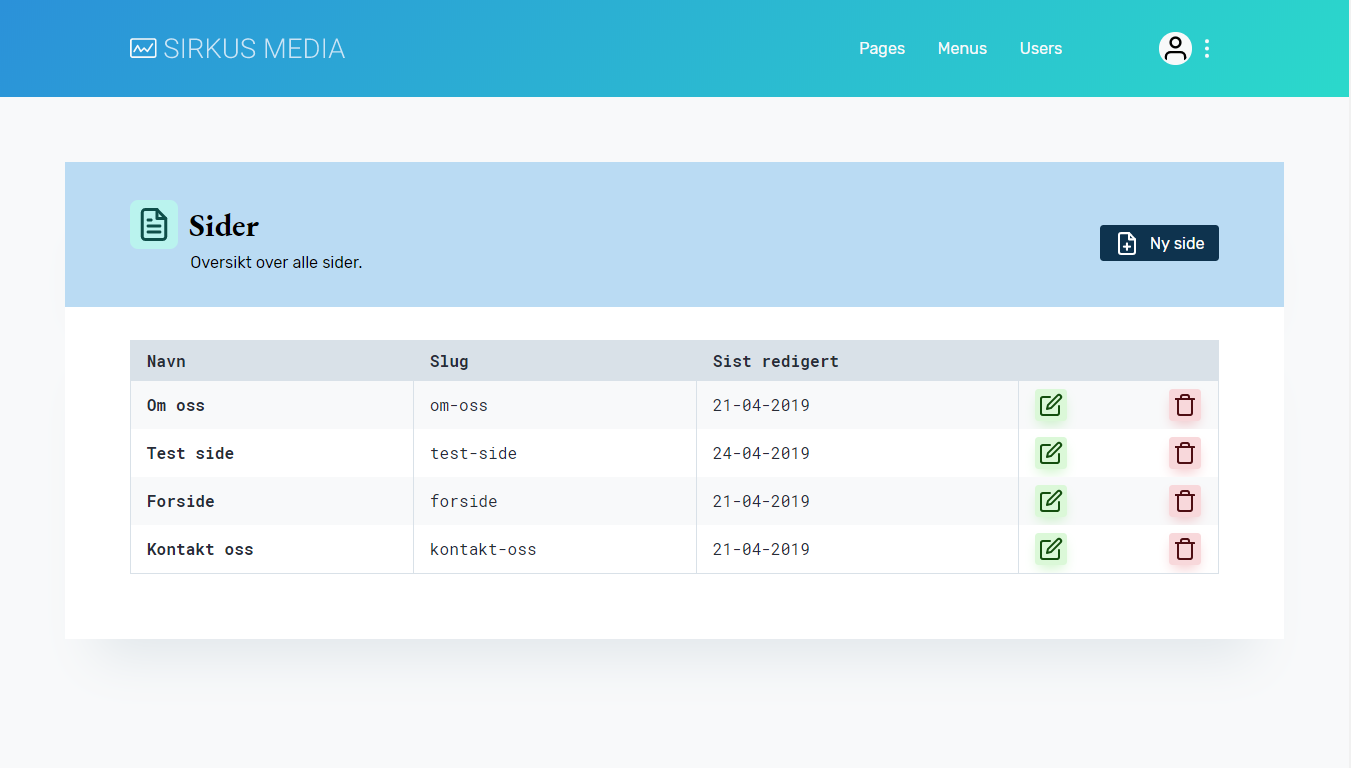
\includegraphics[width=\textwidth]{first-version-cms.png}
    \caption{Første versjon av CMS-et}
    \label{fig:first-version-cms}
\end{figure}

\begin{figure}[H]
    \centering
    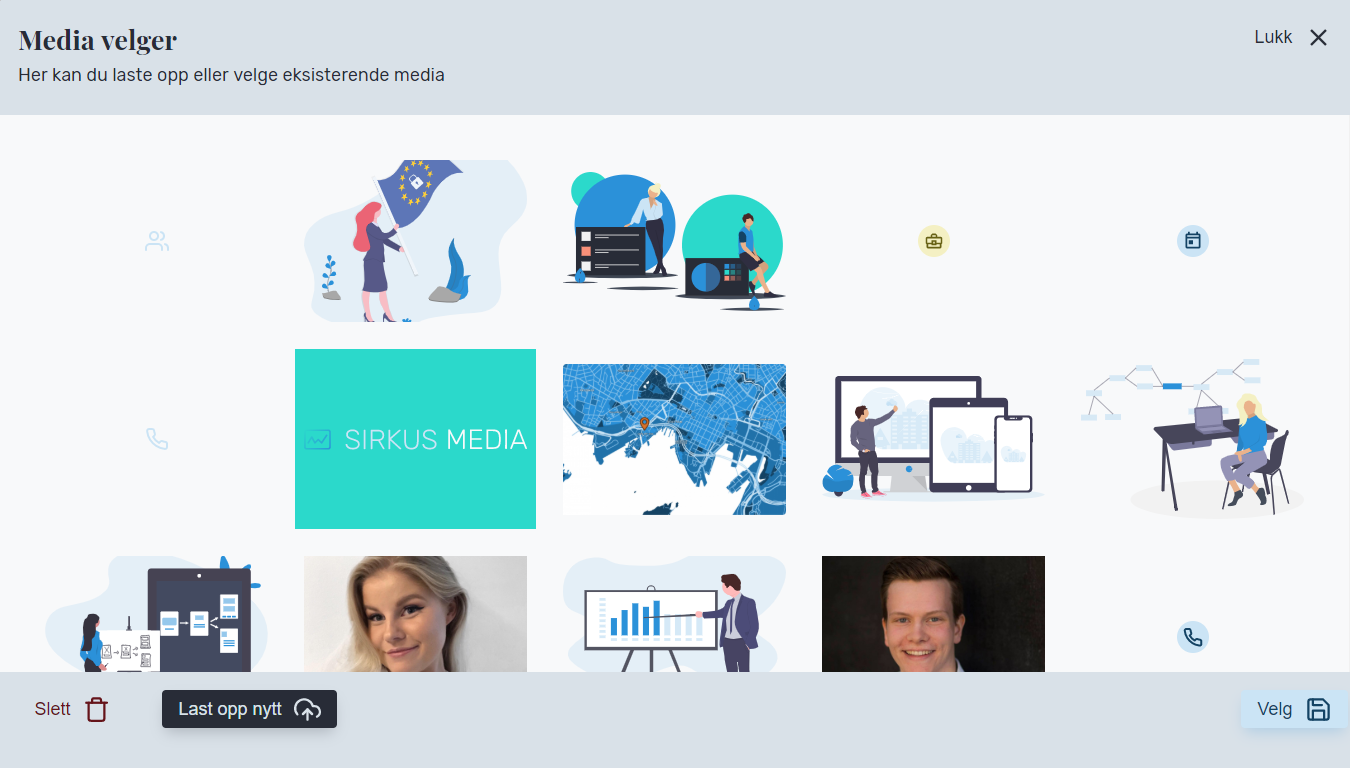
\includegraphics[width=\textwidth]{brukerveiledning/media-picker.png}
    \caption{Bildevelgeren til CMS-et}
    \label{fig:media-picker-cms}
\end{figure}

Nettstedet endte også opp som vi planla i avsnitt \ref{sec:planning-website}. Både forsiden, menyen, om- og kontakt oss siden ble utviklet uten avvik. Videre innholder footeren en link som fører til logg inn til administrasjonsgrensesnittet. Det har også blitt opprettet sider for personvern og informasjonskapsler. Disse innholder tekst fra den opprinnelige nettsiden til oppdragsgiver. Nettstedet består i tillegg av en chat, der meldingene blir sendt direkte til en e-postadresse. Figur \ref{fig:first-version-website} viser første versjon av nettstedet.

\begin{figure}[H]
    \centering
    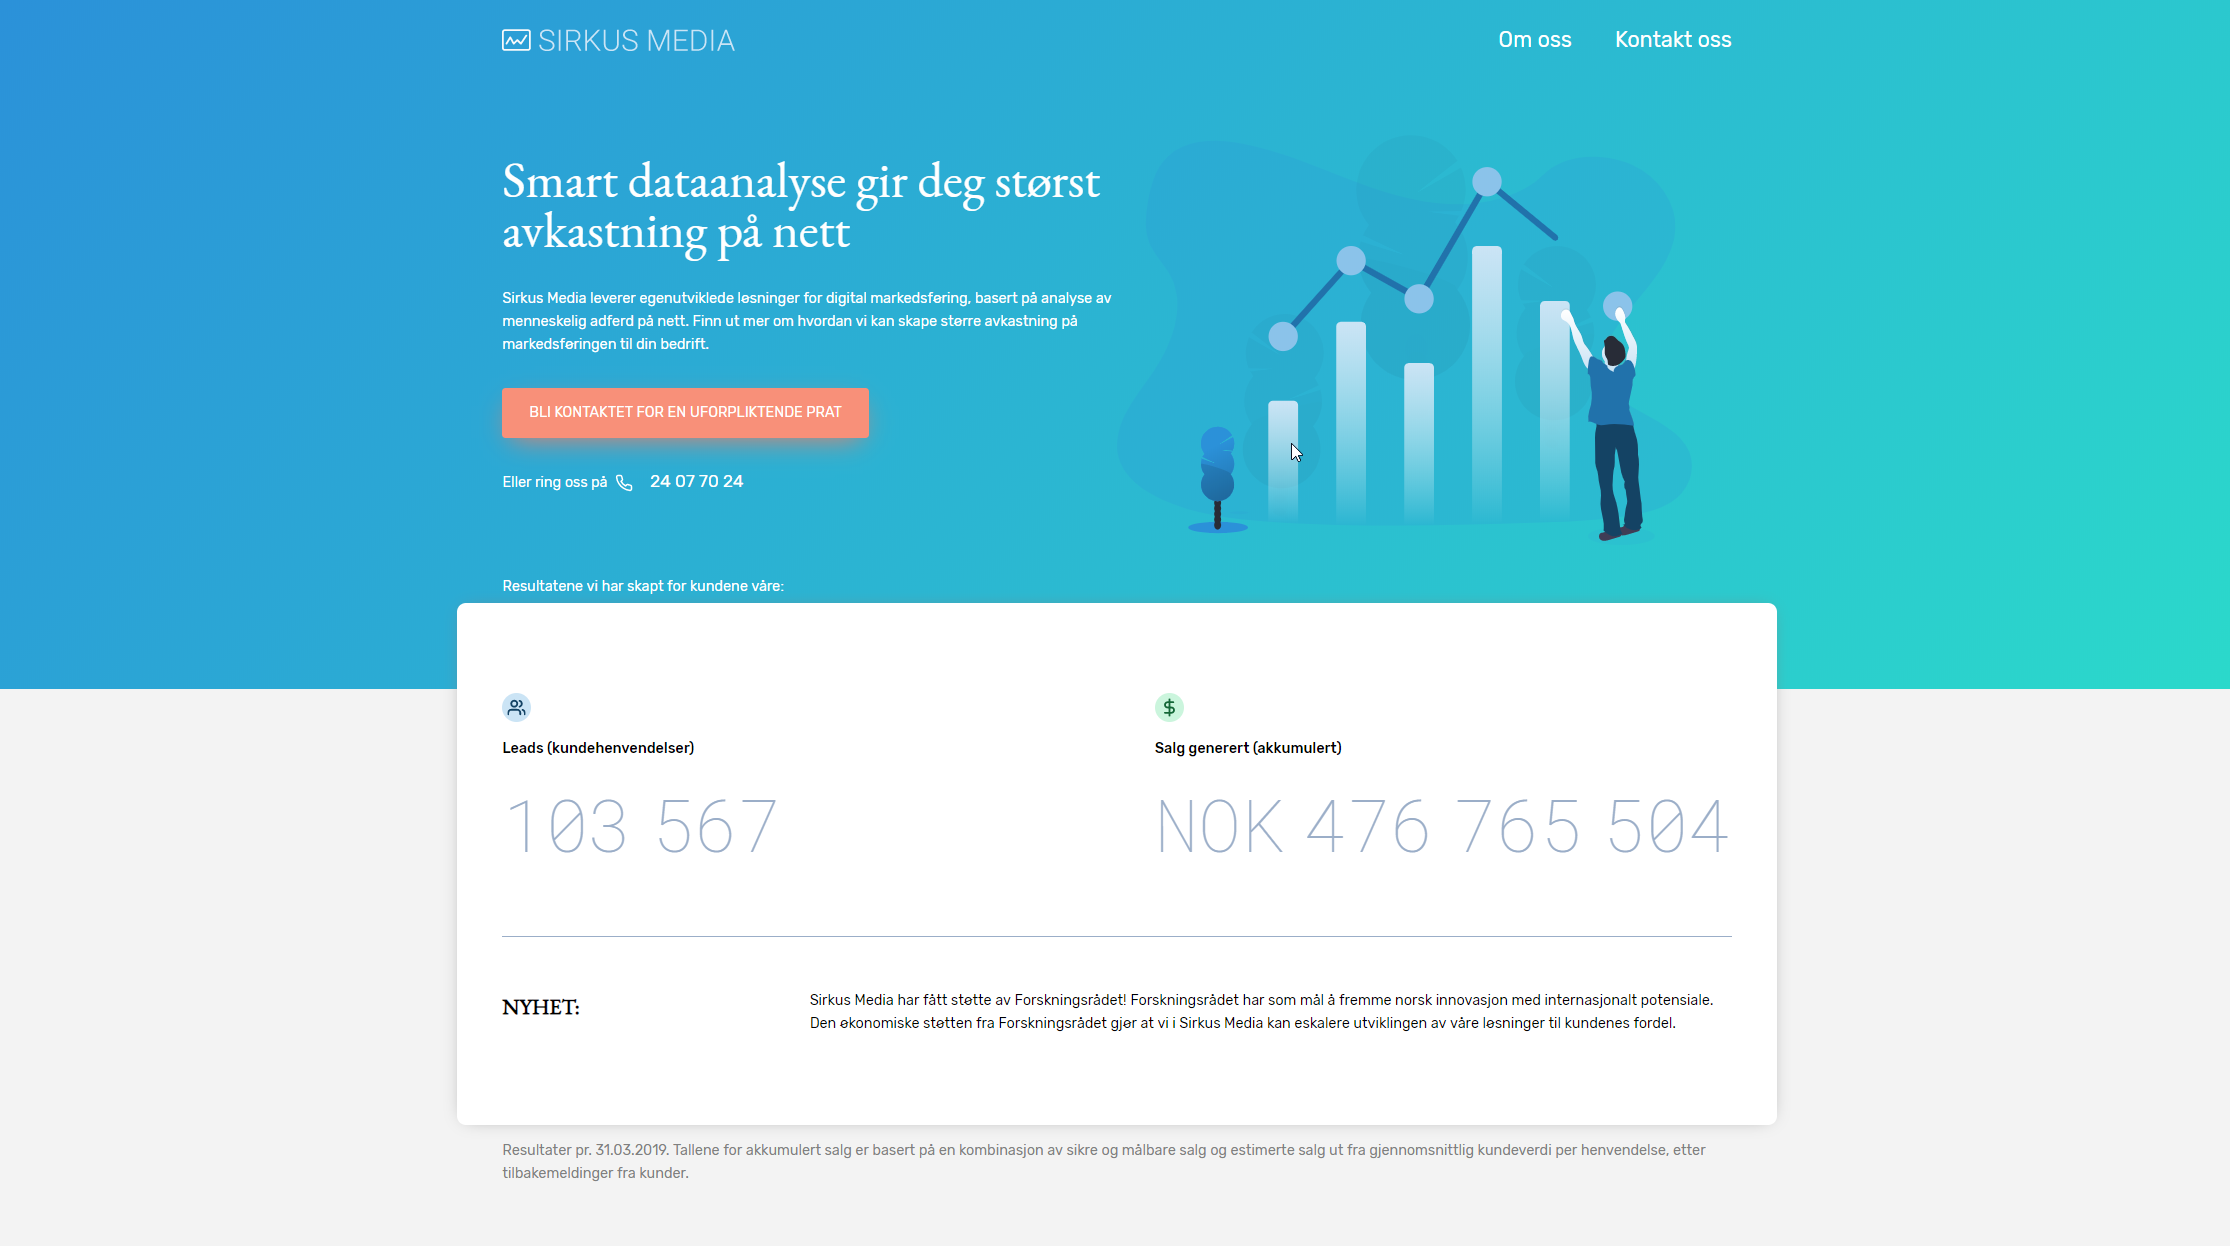
\includegraphics[width=\textwidth]{versjon-1-nettsted.png}
    \caption{Første versjon av nettstedet}
    \label{fig:first-version-website}
\end{figure}